

%
% Introduction: Motivation for this work
%

\begin{frame}{Outline}
 \begin{block}{ViennaCL Overview and Internals}\end{block}
 \begin{block}{Tuning Potpourri: Iterative Solvers}\end{block}
 \begin{block}{Community Building}\end{block}
 \begin{block}{Development Infrastructure}\end{block}
 \begin{block}{Miscellaneous}\end{block}
 \begin{block}{Summary}\end{block}
\end{frame}





%%%%%%%%

\begin{frame}[fragile]
\frametitle{From Boost.uBLAS to ViennaCL}
\begin{block}{Consider Existing CPU Code (Boost.uBLAS)}
  \begin{lstlisting}
using namespace boost::numeric::ublas;


matrix<double> A(1000, 1000);
vector<double> x(1000), y(1000);

/* Fill A, x, y here */

double val = inner_prod(x, y);
y += 2.0 * x;
A += val * outer_prod(x, y);

x = solve(A, y, upper_tag()); // Upper tri. solver

std::cout << "  2-norm: " << norm_2(x) << std::endl;
std::cout << "sup-norm: " << norm_inf(x) << std::endl;
  \end{lstlisting}

  \begin{itemize}
   \item High-level code with syntactic sugar
  \end{itemize}

\end{block}

\end{frame}


\begin{frame}[fragile]
\frametitle{From Boost.uBLAS to ViennaCL}
 \begin{block}{Previous Code Snippet Rewritten with ViennaCL}
  \begin{lstlisting}
using namespace viennacl;
using namespace viennacl::linalg;

matrix<double> A(1000, 1000);
vector<double> x(1000), y(1000);

/* Fill A, x, y here */

double val = inner_prod(x, y);
y += 2.0 * x;
A += val * outer_prod(x, y);

x = solve(A, y, upper_tag()); // Upper tri. solver

std::cout << "  2-norm: " << norm_2(x) << std::endl;
std::cout << "sup-norm: " << norm_inf(x) << std::endl;
  \end{lstlisting} 

  \begin{itemize}
   \item High-level code with syntactic sugar
  \end{itemize}

 \end{block}

\end{frame}



%%%%%%%%%%%%%%% Iterative solvers %%%%%%%%%%%%%%%%%%%%%%
\begin{frame}[fragile]
\frametitle{From Boost.uBLAS to ViennaCL}
\begin{block}{ViennaCL in Addition Provides Iterative Solvers}
  \begin{lstlisting}
using namespace viennacl;
using namespace viennacl::linalg;

compressed_matrix<double> A(1000, 1000);
vector<double> x(1000), y(1000);

/* Fill A, x, y here */

x = solve(A, y, cg_tag());       // Conjugate Gradients
x = solve(A, y, bicgstab_tag()); // BiCGStab solver
x = solve(A, y, gmres_tag());    // GMRES solver
  \end{lstlisting}
\end{block}

 \begin{block}{No Iterative Solvers Available in Boost.uBLAS...}
  \vspace*{1.22cm}
 \end{block}
\end{frame}


\begin{frame}[fragile]
\frametitle{From Boost.uBLAS to ViennaCL}
\begin{block}{Thanks to Interface Compatibility}
  \begin{lstlisting}
using namespace boost::numeric::ublas;
using namespace viennacl::linalg;

compressed_matrix<double> A(1000, 1000);
vector<double> x(1000), y(1000);

/* Fill A, x, y here */

x = solve(A, y, cg_tag());       // Conjugate Gradients
x = solve(A, y, bicgstab_tag()); // BiCGStab solver
x = solve(A, y, gmres_tag());    // GMRES solver
  \end{lstlisting} 
\end{block}

\begin{block}{Code Reuse Beyond GPU Borders}
 \begin{itemize}
  \item Eigen \ { \ \footnotesize \verb|http://eigen.tuxfamily.org/|}
  \item MTL 4 \ { \footnotesize \verb|http://www.mtl4.org/|}
 \end{itemize}
\end{block}

\end{frame}


\begin{frame}[fragile]
\frametitle{From Boost.uBLAS to ViennaCL}
\begin{block}{Generic CG Implementation (Sketch)}
  \begin{lstlisting}
for (unsigned int i = 0; i < tag.max_iterations(); ++i)
{
  tmp = viennacl::linalg::prod(matrix, p);

  alpha     = ip_rr / inner_prod(tmp, p);
  result   += alpha * p;
  residual -= alpha * tmp;
        
  new_ip_rr = inner_prod(residual, residual);
  if (new_ip_rr / norm_rhs_squared < tag.tolerance())
    break;
        
  beta  = new_ip_rr / ip_rr;
  ip_rr = new_ip_rr;

  p = residual + beta * p;
} 
  \end{lstlisting} 
\end{block}

\end{frame}





\begin{frame}[fragile]
\frametitle{From Boost.uBLAS to ViennaCL}
\begin{block}{Yesterday's Vector Addition Tutorial Revisited}
  \begin{lstlisting}
#include <iostream>
#include "viennacl/vector.hpp"

typedef float   NumericT;
using namespace viennacl;

int main()
{
  std::size_t N = 128*1024;
  vector<NumericT> x = scalar_vector<NumericT>(N, 1.0);
  vector<NumericT> y = scalar_vector<NumericT>(N, 2.0);

  x += y;

  std::cout << x << std::endl;
}
  \end{lstlisting} 
\end{block}

\end{frame}




%%%%%%%%%%%%%%%%%%%%%%%%%%%%%%%%%%% ViennaCL %%%%%%%%%%%%%%%%%%%%%%%%%%%%%%%%%%%%

\begin{frame}{About ViennaCL}

  \begin{block}{About}
   \begin{itemize}
    \item High-level linear algebra C++ library
    \item OpenMP, OpenCL, and CUDA backends
    \item Header-only
    \item Multi-platform
   \end{itemize}
  \end{block}

  \vspace*{-2.3cm}
  \begin{flushright}
   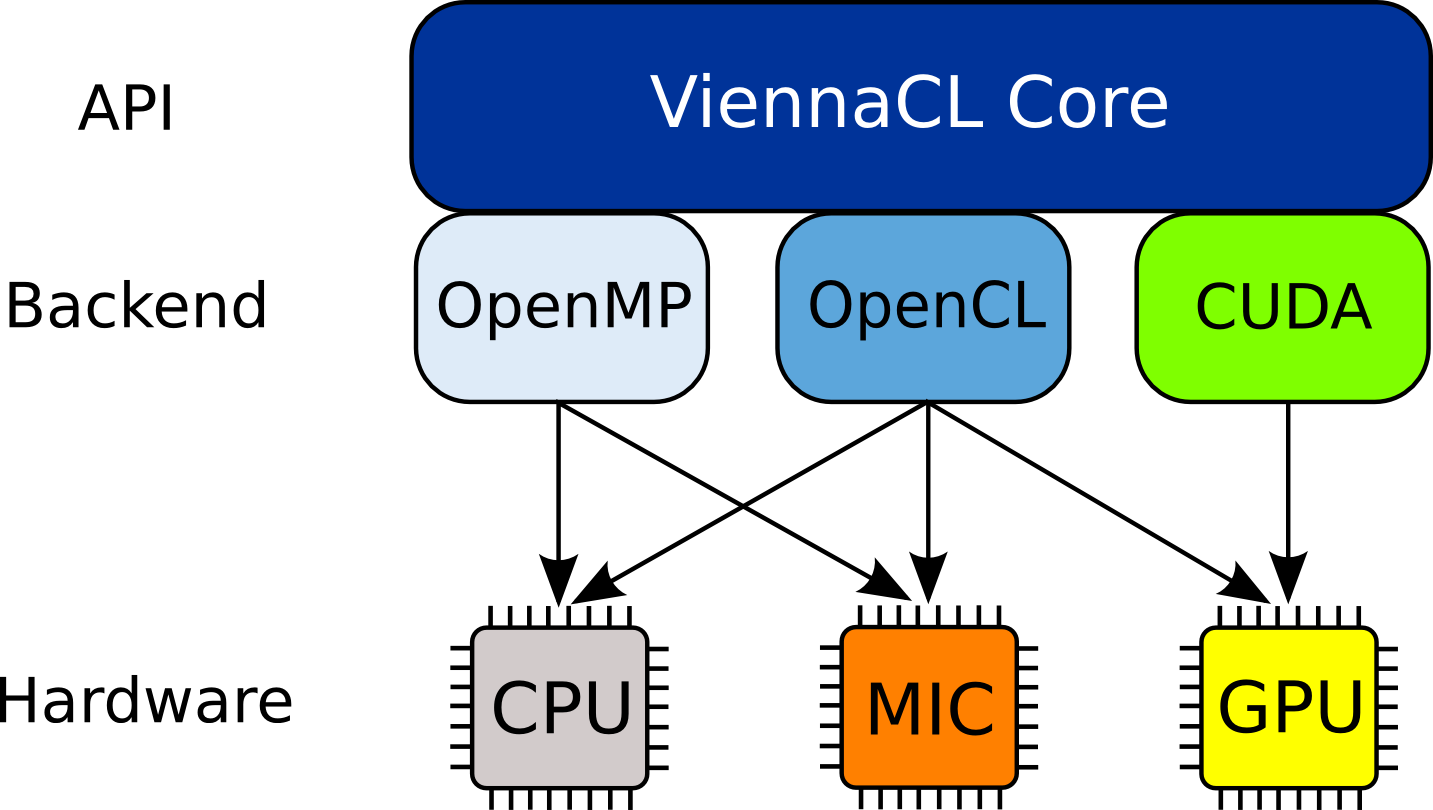
\includegraphics[width=0.4\textwidth]{figures/ViennaCL-arch.png}
  \end{flushright}

  \vspace*{-0.7cm}
  \begin{block}{Dissemination}
    \begin{itemize}
     \item Free Open-Source MIT (X11) License
     \item http://viennacl.sourceforge.net/
     \item 50-100 downloads per week
    \end{itemize}   
  \end{block}

  \begin{block}{Design Rules}
   \begin{itemize}
    \item Reasonable default values
    \item Compatible to Boost.uBLAS whenever possible 
    \item In doubt: clean design over performance
   \end{itemize}
  \end{block}

\end{frame}

%%%%%%%%


%%%%%%%%%%%%%%% Explain ViennaCL types here %%%%%%%%%%%%%%%%%%%%%%

\begin{frame}[fragile]
\frametitle{About ViennaCL}

 \begin{block}{Basic Types}
   \begin{itemize}
    \item scalar
    \item vector
    \item matrix, compressed\_matrix, coordinate\_matrix, ell\_matrix, hyb\_matrix
   \end{itemize}
 \end{block}

 \begin{block}{Data Initialization}
    \begin{itemize}
     \item Using viennacl::copy() 
    \item  { \black
  \begin{lstlisting}
     std::vector<double>      std_x(100);
   ublas::vector<double>    ublas_x(100);
viennacl::vector<double>      vcl_x(100);


for (size_t i=0; i<100; ++i){
    std_x[i] = rand();
  ublas_x[i] = rand();
    vcl_x[i] = rand();  //possible, inefficient
}
  \end{lstlisting} }

%   \item Reuse of C++ STL coding conventions
 \end{itemize}

 \end{block}
\end{frame}



\begin{frame}[fragile]
\frametitle{About ViennaCL}

 \begin{block}{Basic Types}
   \begin{itemize}
    \item scalar
    \item vector
    \item matrix, compressed\_matrix, coordinate\_matrix, ell\_matrix, hyb\_matrix
   \end{itemize}
 \end{block}

 \begin{block}{Data Initialization}
    \begin{itemize}
     \item Using viennacl::copy() 
    \item  { \black
  \begin{lstlisting}
     std::vector<double>      std_x(100);
   ublas::vector<double>    ublas_x(100);
viennacl::vector<double>      vcl_x(100);

/* setup of std_x and ublas_x omitted */

viennacl::copy(std_x.begin(), std_x.end(),
               vcl_x.begin());   //to GPU
viennacl::copy(vcl_x.begin(), vcl_x.end(),
               ublas_x.begin()); //to CPU
  \end{lstlisting} }

%   \item Reuse of C++ STL coding conventions
 \end{itemize}

 \end{block}
\end{frame}


\begin{frame}[fragile]
\frametitle{About ViennaCL}

 \begin{block}{Basic Types}
   \begin{itemize}
    \item scalar
    \item vector
    \item matrix, compressed\_matrix, coordinate\_matrix, ell\_matrix, hyb\_matrix
   \end{itemize}
 \end{block}

 \begin{block}{Data Initialization}
    \begin{itemize}
     \item Using viennacl::copy() 
    \item  { \black
  \begin{lstlisting}
     std::vector<std::vector<double> >    std_A;
   ublas::matrix<double>                ublas_A;
viennacl::matrix<double>                  vcl_A;

/* setup of std_A and ublas_A omitted */

viennacl::copy(std_A,
               vcl_A);    // CPU to GPU
viennacl::copy(vcl_A,
               ublas_A);  // GPU to CPU
  \end{lstlisting} }
 \end{itemize}

 \end{block}
\end{frame}







\begin{frame}[fragile]
\frametitle{Internals}

 \begin{block}{Vector Addition}
  \begin{lstlisting}
 x = y + z;
  \end{lstlisting}
 \end{block}

  %\pause

 \begin{block}{Naive Operator Overloading}
  \begin{lstlisting}
 vector<T> operator+(vector<T> & v, vector<T> & w);
  \end{lstlisting}

  %\pause

  \begin{itemize}
   \item t $\leftarrow$ y + z, x $\leftarrow$ t
   %\pause
   \item Temporaries are extremely expensive! 
  \end{itemize}
 \end{block}

   %\pause

 \begin{block}{Expression Templates}
  \begin{lstlisting}
 vector_expr<vector<T>, op_plus, vector<T> >
 operator+(vector<T> & v, vector<T> & w) { ... }

 vector::operator=(vector_expr<...> const & e) {
   viennacl::linalg::avbv(*this, 1,e.lhs(), 1,e.rhs());
 }
  \end{lstlisting}
  \vspace*{0.5cm}

 \end{block}

\end{frame}



\begin{frame}[fragile]
\frametitle{Internals}

 \begin{block}{Vector Addition}
  \begin{lstlisting}
// x = y + z
void avbv(...) {
  switch (active_handle_id(x))
  {
    case MAIN_MEMORY:
      host_based::avbv(...);
      break;
    case OPENCL_MEMORY:
      opencl::avbv(...);
      break;
    case CUDA_MEMORY:
      cuda::avbv(...);
      break;
    default: 
      raise_error();
  }
}
\end{lstlisting}
  \begin{itemize}
   \item Memory buffers can switch memory domain at runtime
  \end{itemize}

 \end{block}

\end{frame}

\begin{frame}[fragile]
\frametitle{Internals}

 \begin{block}{Memory Buffer Migration}
  \begin{lstlisting}
  vector<double> x = zero_vector<double>(42);

  memory_types src_memory_loc = memory_domain(x);
  switch_memory_domain(x, MAIN_MEMORY);

  /* do work on x in main memory here */

  switch_memory_domain(x, src_memory_loc);
\end{lstlisting}

  \begin{center}
    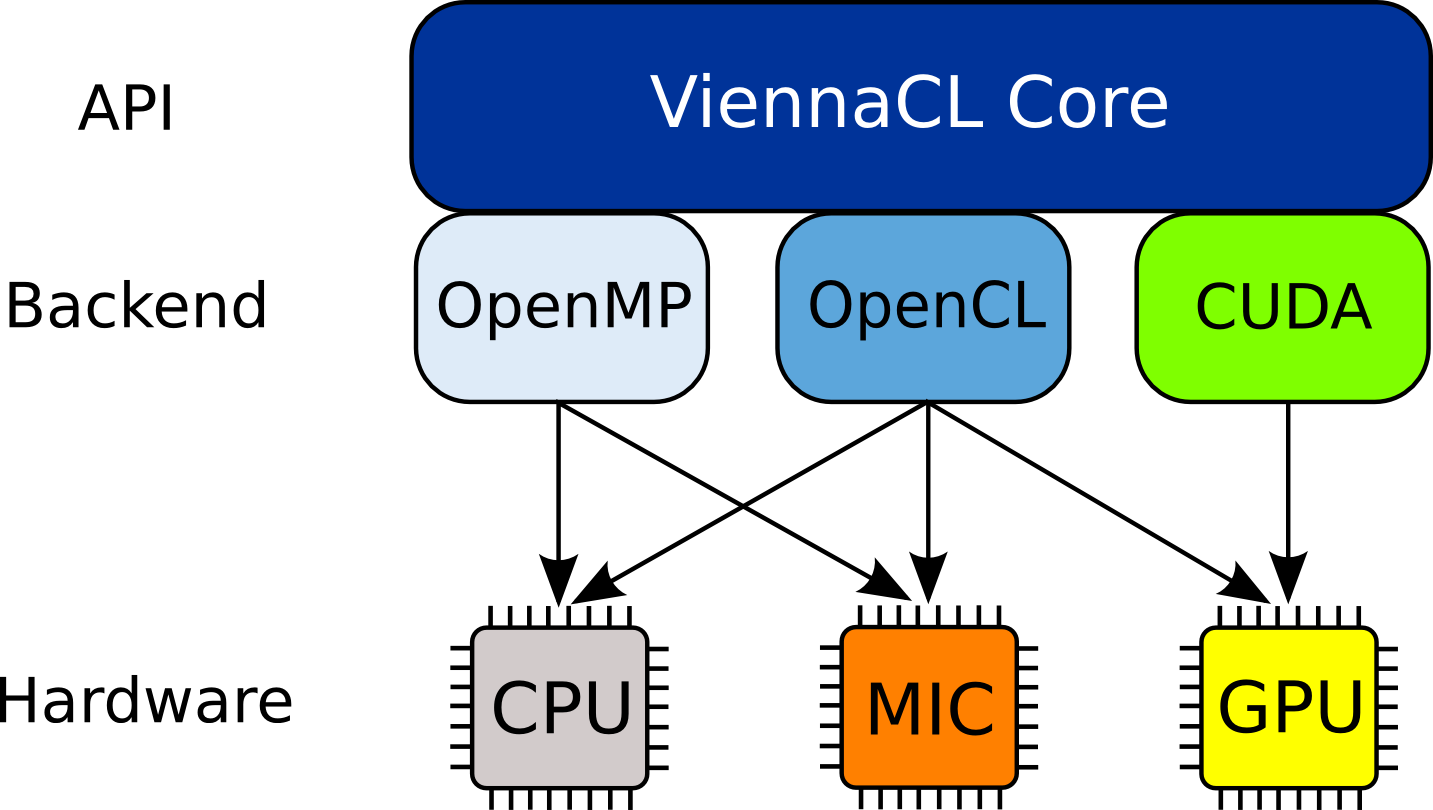
\includegraphics[width=0.6\textwidth]{figures/ViennaCL-arch.png}
  \end{center}
 \end{block}

\end{frame}




\begin{frame}[fragile]
\frametitle{Internals}

 \begin{block}{Generalizing compute kernels}
  \begin{lstlisting}
  // x = y + z
  __kernel void avbv(
    double * x,

    double * y,

    double * z, uint size)
{
  i = get_global_id(0);
  for (size_t i=0; i<size; i += get_global_size())
    x[i] = y[i] + z[i]; 

}
  \end{lstlisting}
 \end{block}

 \vspace*{1.5cm}
\end{frame}



\begin{frame}[fragile]
\frametitle{Internals}

 \begin{block}{Generalizing compute kernels}
  \begin{lstlisting}
  // x = a * y + b * z
  __kernel void avbv(
    double * x,
    double a,
    double * y,
    double b,
    double * z, uint size)
{
  i = get_global_id(0);
  for (size_t i=0; i<size; i += get_global_size())
    x[i] = a * y[i] + b * z[i]; 

}
  \end{lstlisting}
 \end{block}

 \vspace*{1.5cm}
\end{frame}


\begin{frame}[fragile]
\frametitle{Internals}

 \begin{block}{Generalizing compute kernels}
  \begin{lstlisting}
  // x[4:8] = a * y[2:6] + b * z[3:7]
  __kernel void avbv(
    double * x, uint off_x,
    double a,
    double * y, uint off_y,
    double b,
    double * z, uint off_z, uint size)
{
  i = get_global_id(0);
  for (size_t i=0; i<size; i += get_global_size())
    x[off_x + i] = a * y[off_y + i] + b * z[off_z + i]; 

}
  \end{lstlisting}
 \end{block}

 \vspace*{1.5cm}
\end{frame}



\begin{frame}[fragile]
\frametitle{Internals}

 \begin{block}{Generalizing compute kernels}
  \begin{lstlisting}
  // x[4:2:8] = a * y[2:2:6] + b * z[3:2:7]
  __kernel void avbv(
    double * x, uint off_x, uint inc_x,
    double a,
    double * y, uint off_y, uint inc_y,
    double b,
    double * z, uint off_z, uint inc_z, uint size)
{
  i = get_global_id(0);
  for (size_t i=0; i<size; i += get_global_size())
    x[off_x + i * inc_x] =  a * y[off_y + i * inc_y]
                          + b * z[off_z + i * inc_z]; 
}
  \end{lstlisting}
 \end{block}

  \begin{block}{}
   \begin{itemize}
    \item No penalty on GPUs because FLOPs are for free
   \end{itemize}
  \end{block}

\end{frame}





\begin{frame}{Outline}
 \begin{block}{ViennaCL Overview and Internals}\end{block}
 \begin{block}{\textbf{Tuning Potpourri: Iterative Solvers}}\end{block}
 \begin{block}{Community Building}\end{block}
 \begin{block}{Development Infrastructure}\end{block}
 \begin{block}{Miscellaneous}\end{block}
 \begin{block}{Summary}\end{block}
\end{frame}


%
% Introduce CG and perform first optimizations
%


%%
%% Conjugate Gradients: Pipelining
%%

% Show CG algorithm <-> BLAS


\begin{frame}[fragile]{Performance Modeling: Conjugate Gradients}

 \begin{block}{}
  
   \begin{minipage}{0.45\textwidth}
      {\large \textbf{Pseudocode}} \\
      
      Choose $x_0$ \\
      $p_0 = r_0 = b - Ax_0$ \\
      For $i=0$ until convergence
     \begin{enumerate}
      \item Compute and store $Ap_i$
      \item Compute $\langle p_i, Ap_i \rangle$
      \item $\alpha_i = \langle r_i, r_i \rangle / \langle p_i, Ap_i \rangle$
      \item $x_{i+1} = x_{i} + \alpha_i p_i$          
      \item $r_{i+1} = r_i - \alpha_i Ap_i$       
      \item Compute $\langle r_{i+1}, r_{i+1} \rangle$
      \item $\beta_i = \langle r_{i+1}, r_{i+1} \rangle / \langle r_i, r_i \rangle$
      \item $p_{i+1} = r_{i+1} + \beta_i p_i$
     \end{enumerate}
     EndFor
   \end{minipage}
   \begin{minipage}{0.48\textwidth}
      {\large \textbf{BLAS-based Implementation}} \\
      
            - \\
      SpMV, AXPY \\
      For $i=0$ until convergence
     \begin{enumerate}
      \item SpMV {\color{blue} $\leftarrow$ No caching of $Ap_i$}
      \item DOT {\color{red} $\leftarrow$ Global sync!}
      \item -
      \item AXPY         
      \item AXPY  {\color{blue} $\leftarrow$ No caching of $r_{i+1}$}
      \item DOT {\color{red} $\leftarrow$ Global sync!}
      \item -
      \item AXPY
     \end{enumerate}
     EndFor
   \end{minipage}
   
   \end{block}
   
\end{frame}

\begin{frame}[fragile]{Performance Modeling: Conjugate Gradients}

 \begin{block}{}
 
 \begin{center}
  \vspace*{-0.5cm}
  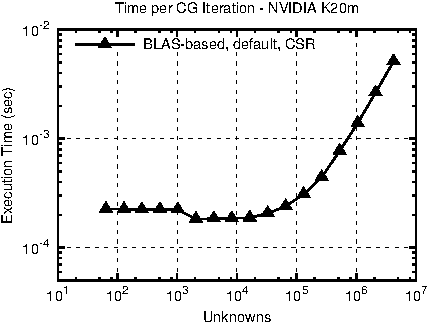
\includegraphics[width=0.85\textwidth]{figures/cg-k20m-0}
 \end{center}

 \begin{itemize}
  \item   \vspace*{-0.3cm} {\small (Poisson, 2D, Finite Differences)}
 \end{itemize}

 \end{block}
   
\end{frame}


\begin{frame}[fragile]{Performance Modeling: Conjugate Gradients}

 \begin{block}{Performance Modelling}
   \begin{itemize}
    \item 6 Kernel Launches (plus two for reductions)
    \item Two device to host data reads from dot products
    \item Model SpMV as seven vector accesses (5-point stencil)
    \item $T(N) = 8 \times 10^{-6} + 2 \times 2 \times 10^{-6} + (7+2+3+3+2+3) \times 8 \times N / \mathrm{Bandwidth}$
   \end{itemize}

 %\pause
 \begin{center}
  \vspace*{-0.2cm}
  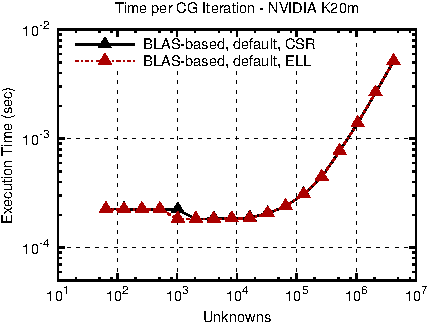
\includegraphics[width=0.65\textwidth]{figures/cg-k20m-1}
 \end{center}

%  \begin{itemize}
%   \item   \vspace*{-0.5cm} {\small (Poisson, 2D, Finite Differences)}
%  \end{itemize}

 \end{block}
   
\end{frame}


%%%%%%%%

% Step 3: Show and discuss pipelined/improved version

\begin{frame}[fragile]{Performance Modeling: Conjugate Gradient Optimizations}

 \begin{block}{Optimization: Rearrange the algorithm}
   \begin{itemize}
   \item  Remove unnecessary reads 
   \item  Remove unnecessary synchronizations
   \item Use custom kernels instead of standard BLAS
  \end{itemize}
 \end{block}
   
\end{frame}



\begin{frame}[fragile]{Performance Modeling: Conjugate Gradients}

 \begin{block}{}
  
   \begin{minipage}{0.45\textwidth}
      {\large \textbf{Standard CG}} \\
      
      Choose $x_0$ \\
      $p_0 = r_0 = b - Ax_0$ \\
      For $i=0$ until convergence
     \begin{enumerate}
      \item Compute and store $Ap_i$
      \item Compute $\langle p_i, Ap_i \rangle$
      \item $\alpha_i = \langle r_i, r_i \rangle / \langle p_i, Ap_i \rangle$
      \item $x_{i+1} = x_{i} + \alpha_i p_i$          
      \item $r_{i+1} = r_i - \alpha_i Ap_i$       
      \item Compute $\langle r_{i+1}, r_{i+1} \rangle$
      \item $\beta_i = \langle r_{i+1}, r_{i+1} \rangle / \langle r_i, r_i \rangle$
      \item $p_{i+1} = r_{i+1} + \beta_i p_i$
     \end{enumerate}
     EndFor
   \end{minipage}
   \begin{minipage}{0.53\textwidth}
      {\large \textbf{Pipelined CG}} \\
      
      Choose $x_0$ \\
      $p_0 = r_0 = b - Ax_0$ \\
      For $i=1$ until convergence
     \begin{enumerate}
      \item $i=1$: Compute $\alpha_0$, $\beta_0$, $Ap_0$
      \item {\color{blue}$x_i = x_{i-1} + \alpha_{i-1} p_{i-1}$}
      \item {\color{blue}$r_i = r_{i-1} - \alpha_{i-1} Ap_i$}
      \item {\color{blue}$p_i = r_i + \beta_{i-1} p_{i-1}$}       
      \item {\color{red} Compute and store $Ap_i$}
      \item  {\color{red} Compute $\langle Ap_i, Ap_i \rangle$, $\langle p_i, Ap_i \rangle$}, {\color{blue}$\langle r_i, r_i \rangle$}
      \item $\alpha_i = \langle r_i, r_i \rangle / \langle p_i, Ap_i \rangle$
      \item $\beta_i = ( \alpha_i^2 \langle Ap_i, Ap_i \rangle - \langle r_i, r_i \rangle) / \langle r_i, r_i \rangle$
     \end{enumerate}
     EndFor
   \end{minipage}
   
   \end{block}
   
\end{frame}


\begin{frame}[fragile]{Performance Modeling: Conjugate Gradients}
 \begin{block}{}
 \begin{center}
  \vspace*{-0.5cm}
  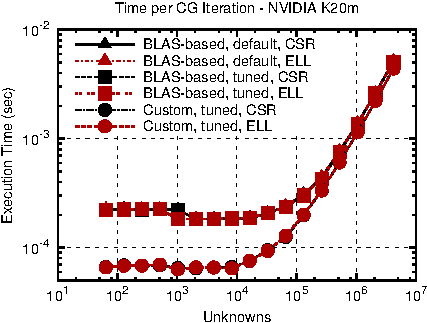
\includegraphics[width=0.85\textwidth]{figures/cg-k20m-3}
 \end{center}

 \begin{itemize}
  \item   \vspace*{-0.3cm} {\small (Poisson, 2D, Finite Differences)}
 \end{itemize}
 \end{block}   
\end{frame}



\begin{frame}[fragile]{Performance Modeling: Conjugate Gradients}
 \begin{block}{Benefits of Pipelining also for Large Matrices}
 \begin{center}
  \vspace*{-0.2cm}
  \hspace*{-1.5cm}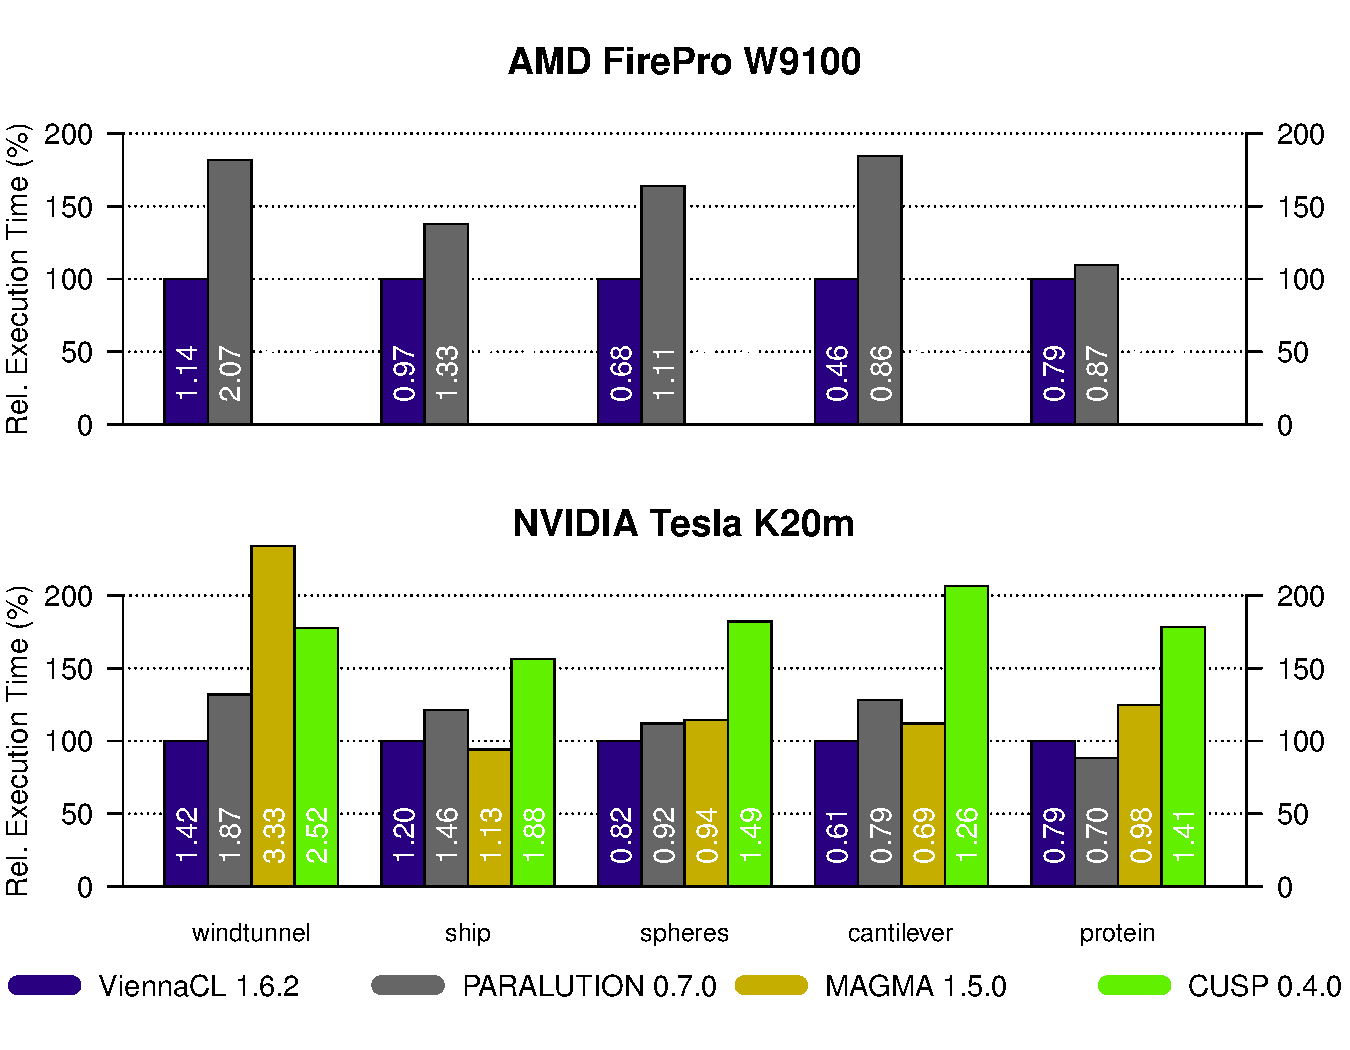
\includegraphics[width=1.05\textwidth]{figures/cg}
 \end{center}
  \vspace*{0.2cm}

 \end{block}   
\end{frame}





%
% Continue with CG-method, show results for pipelined variant
%


\begin{frame}{Outline}
 \begin{center}
  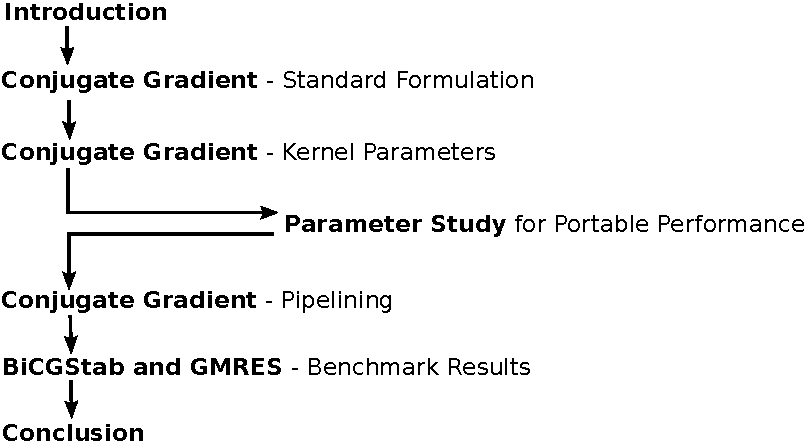
\includegraphics[width=0.9\textwidth]{figures/outline-crop}
 \end{center}
\end{frame}

\begin{frame}[fragile]{Conjugate Gradients}
 \begin{block}{}
 \begin{center}
  \vspace*{-0.5cm}
  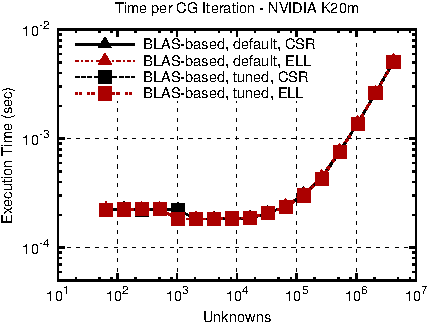
\includegraphics[width=0.85\textwidth]{figures/cg-k20m-2}
 \end{center}

 \begin{itemize}
  \item   \vspace*{-0.3cm} {\small (2D Finite Difference Discretization)}
 \end{itemize}
 \end{block}   
\end{frame}

\begin{frame}[fragile]{Conjugate Gradients}
 \begin{block}{}
 \begin{center}
  \vspace*{-0.5cm}
  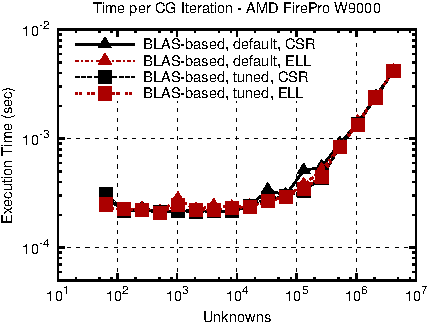
\includegraphics[width=0.85\textwidth]{figures/cg-firepro-w9000-2}
 \end{center}

 \begin{itemize}
  \item   \vspace*{-0.3cm} {\small (2D Finite Difference Discretization)}
 \end{itemize}
 \end{block}   
\end{frame}


% Step 3: Show and discuss pipelined/improved version

\begin{frame}[fragile]{Conjugate Gradient Optimizations}

 \begin{block}{Optimization 3: Rearrange the algorithm}
   \begin{itemize}
   \item  Remove unnecessary reads 
   \item  Remove unnecessary synchronizations
   \item Use custom kernels instead of standard BLAS
  \end{itemize}
 \end{block}
   
\end{frame}


\begin{frame}[fragile]{Conjugate Gradients}

 \begin{block}{}
  
   \begin{minipage}{0.45\textwidth}
      {\large \textbf{Standard CG}} \\
      
      Choose $x_0$ \\
      $p_0 = r_0 = b - Ax_0$ \\
      For $i=0$ until convergence
     \begin{enumerate}
      \item Compute and store $Ap_i$
      \item Compute $\langle p_i, Ap_i \rangle$
      \item $\alpha_i = \langle r_i, r_i \rangle / \langle p_i, Ap_i \rangle$
      \item $x_{i+1} = x_{i} + \alpha_i p_i$          
      \item $r_{i+1} = r_i - \alpha_i Ap_i$       
      \item Compute $\langle r_{i+1}, r_{i+1} \rangle$
      \item $\beta_i = \langle r_{i+1}, r_{i+1} \rangle / \langle r_i, r_i \rangle$
      \item $p_{i+1} = r_{i+1} + \beta_i p_i$
     \end{enumerate}
     EndFor
   \end{minipage}
   \begin{minipage}{0.53\textwidth}
   \end{minipage}
   
   \end{block}
   
\end{frame}


\begin{frame}[fragile]{Conjugate Gradients}

 \begin{block}{}
  
   \begin{minipage}{0.45\textwidth}
      {\large \textbf{Standard CG}} \\
      
      Choose $x_0$ \\
      $p_0 = r_0 = b - Ax_0$ \\
      For $i=0$ until convergence
     \begin{enumerate}
      \item Compute and store $Ap_i$
      \item Compute $\langle p_i, Ap_i \rangle$
      \item $\alpha_i = \langle r_i, r_i \rangle / \langle p_i, Ap_i \rangle$
      \item $x_{i+1} = x_{i} + \alpha_i p_i$          
      \item $r_{i+1} = r_i - \alpha_i Ap_i$       
      \item Compute $\langle r_{i+1}, r_{i+1} \rangle$
      \item $\beta_i = \langle r_{i+1}, r_{i+1} \rangle / \langle r_i, r_i \rangle$
      \item $p_{i+1} = r_{i+1} + \beta_i p_i$
     \end{enumerate}
     EndFor
   \end{minipage}
   \begin{minipage}{0.53\textwidth}
      {\large \textbf{Pipelined CG}} \\
      
      Choose $x_0$ \\
      $p_0 = r_0 = b - Ax_0$ \\
      For $i=1$ until convergence
     \begin{enumerate}
      \item $i=1$: Compute $\alpha_0$, $\beta_0$, $Ap_0$
      \item $x_i = x_{i-1} + \alpha_{i-1} p_{i-1}$          
      \item $r_i = r_{i-1} - \alpha_{i-1} Ap_i$       
      \item $p_i = r_i + \beta_{i-1} p_{i-1}$       
      \item Compute and store $Ap_i$
      \item Compute $\langle Ap_i, Ap_i \rangle$, $\langle p_i, Ap_i \rangle$, $\langle r_i, r_i \rangle$
      \item $\alpha_i = \langle r_i, r_i \rangle / \langle p_i, Ap_i \rangle$
      \item $\beta_i = ( \alpha_i^2 \langle Ap_i, Ap_i \rangle - \langle r_i, r_i \rangle) / \langle r_i, r_i \rangle$
     \end{enumerate}
     EndFor
   \end{minipage}
   
   \end{block}
   
\end{frame}

\begin{frame}[fragile]{Conjugate Gradients}

 \begin{block}{}
  
   \begin{minipage}{0.45\textwidth}
      {\large \textbf{Standard CG}} \\
      
      Choose $x_0$ \\
      $p_0 = r_0 = b - Ax_0$ \\
      For $i=0$ until convergence
     \begin{enumerate}
      \item Compute and store $Ap_i$
      \item Compute $\langle p_i, Ap_i \rangle$
      \item $\alpha_i = \langle r_i, r_i \rangle / \langle p_i, Ap_i \rangle$
      \item $x_{i+1} = x_{i} + \alpha_i p_i$          
      \item $r_{i+1} = r_i - \alpha_i Ap_i$       
      \item Compute $\langle r_{i+1}, r_{i+1} \rangle$
      \item $\beta_i = \langle r_{i+1}, r_{i+1} \rangle / \langle r_i, r_i \rangle$
      \item $p_{i+1} = r_{i+1} + \beta_i p_i$
     \end{enumerate}
     EndFor
   \end{minipage}
   \begin{minipage}{0.53\textwidth}
      {\large \textbf{Pipelined CG}} \\
      
      Choose $x_0$ \\
      $p_0 = r_0 = b - Ax_0$ \\
      For $i=1$ until convergence
     \begin{enumerate}
      \item $i=1$: Compute $\alpha_0$, $\beta_0$, $Ap_0$
      \item {\color{blue}$x_i = x_{i-1} + \alpha_{i-1} p_{i-1}$}
      \item {\color{blue}$r_i = r_{i-1} - \alpha_{i-1} Ap_i$}
      \item {\color{blue}$p_i = r_i + \beta_{i-1} p_{i-1}$}       
      \item Compute and store $Ap_i$
      \item Compute $\langle Ap_i, Ap_i \rangle$, $\langle p_i, Ap_i \rangle$, {\color{blue}$\langle r_i, r_i \rangle$}
      \item $\alpha_i = \langle r_i, r_i \rangle / \langle p_i, Ap_i \rangle$
      \item $\beta_i = ( \alpha_i^2 \langle Ap_i, Ap_i \rangle - \langle r_i, r_i \rangle) / \langle r_i, r_i \rangle$
     \end{enumerate}
     EndFor
   \end{minipage}
   
   \end{block}
   
\end{frame}


\begin{frame}[fragile]{Conjugate Gradients}

 \begin{block}{}
  
   \begin{minipage}{0.45\textwidth}
      {\large \textbf{Standard CG}} \\
      
      Choose $x_0$ \\
      $p_0 = r_0 = b - Ax_0$ \\
      For $i=0$ until convergence
     \begin{enumerate}
      \item Compute and store $Ap_i$
      \item Compute $\langle p_i, Ap_i \rangle$
      \item $\alpha_i = \langle r_i, r_i \rangle / \langle p_i, Ap_i \rangle$
      \item $x_{i+1} = x_{i} + \alpha_i p_i$          
      \item $r_{i+1} = r_i - \alpha_i Ap_i$       
      \item Compute $\langle r_{i+1}, r_{i+1} \rangle$
      \item $\beta_i = \langle r_{i+1}, r_{i+1} \rangle / \langle r_i, r_i \rangle$
      \item $p_{i+1} = r_{i+1} + \beta_i p_i$
     \end{enumerate}
     EndFor
   \end{minipage}
   \begin{minipage}{0.53\textwidth}
      {\large \textbf{Pipelined CG}} \\
      
      Choose $x_0$ \\
      $p_0 = r_0 = b - Ax_0$ \\
      For $i=1$ until convergence
     \begin{enumerate}
      \item $i=1$: Compute $\alpha_0$, $\beta_0$, $Ap_0$
      \item {\color{blue}$x_i = x_{i-1} + \alpha_{i-1} p_{i-1}$}
      \item {\color{blue}$r_i = r_{i-1} - \alpha_{i-1} Ap_i$}
      \item {\color{blue}$p_i = r_i + \beta_{i-1} p_{i-1}$}       
      \item {\color{red} Compute and store $Ap_i$}
      \item  {\color{red} Compute $\langle Ap_i, Ap_i \rangle$, $\langle p_i, Ap_i \rangle$}, {\color{blue}$\langle r_i, r_i \rangle$}
      \item $\alpha_i = \langle r_i, r_i \rangle / \langle p_i, Ap_i \rangle$
      \item $\beta_i = ( \alpha_i^2 \langle Ap_i, Ap_i \rangle - \langle r_i, r_i \rangle) / \langle r_i, r_i \rangle$
     \end{enumerate}
     EndFor
   \end{minipage}
   
   \end{block}
   
\end{frame}


\begin{frame}[fragile]{Conjugate Gradients}
 \begin{block}{}
 \begin{center}
  \vspace*{-0.5cm}
  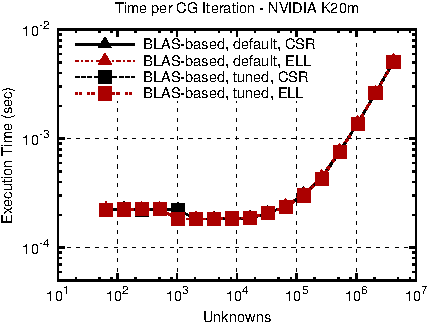
\includegraphics[width=0.85\textwidth]{figures/cg-k20m-2}
 \end{center}

 \begin{itemize}
  \item   \vspace*{-0.3cm} {\small (2D Finite Difference Discretization)}
 \end{itemize}
 \end{block}   
\end{frame}

\begin{frame}[fragile]{Conjugate Gradients}
 \begin{block}{}
 \begin{center}
  \vspace*{-0.5cm}
  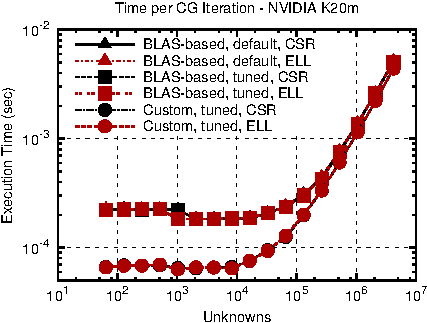
\includegraphics[width=0.85\textwidth]{figures/cg-k20m-3}
 \end{center}

 \begin{itemize}
  \item   \vspace*{-0.3cm} {\small (2D Finite Difference Discretization)}
 \end{itemize}
 \end{block}   
\end{frame}

\begin{frame}[fragile]{Conjugate Gradients}
 \begin{block}{}
 \begin{center}
  \vspace*{-0.5cm}
  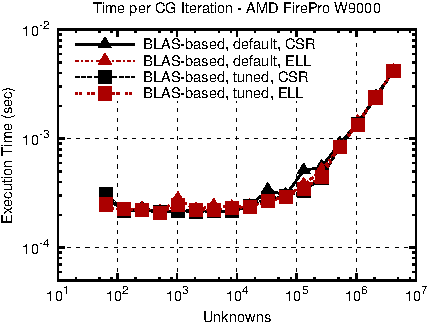
\includegraphics[width=0.85\textwidth]{figures/cg-firepro-w9000-2}
 \end{center}

 \begin{itemize}
  \item   \vspace*{-0.3cm} {\small (2D Finite Difference Discretization)}
 \end{itemize}
 \end{block}   
\end{frame}

\begin{frame}[fragile]{Conjugate Gradients}
 \begin{block}{}
 \begin{center}
  \vspace*{-0.5cm}
  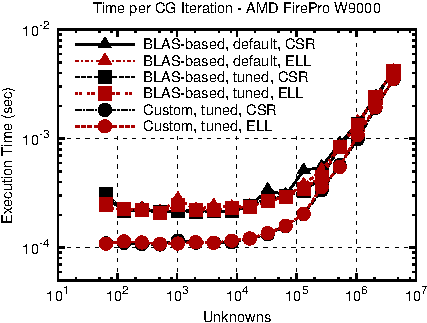
\includegraphics[width=0.85\textwidth]{figures/cg-firepro-w9000-3}
 \end{center}

 \begin{itemize}
  \item   \vspace*{-0.3cm} {\small (2D Finite Difference Discretization)}
 \end{itemize}
 \end{block}   
\end{frame}



%%% BiCGStab and GMRES optimization:


\begin{frame}{Outline}
 \begin{center}
  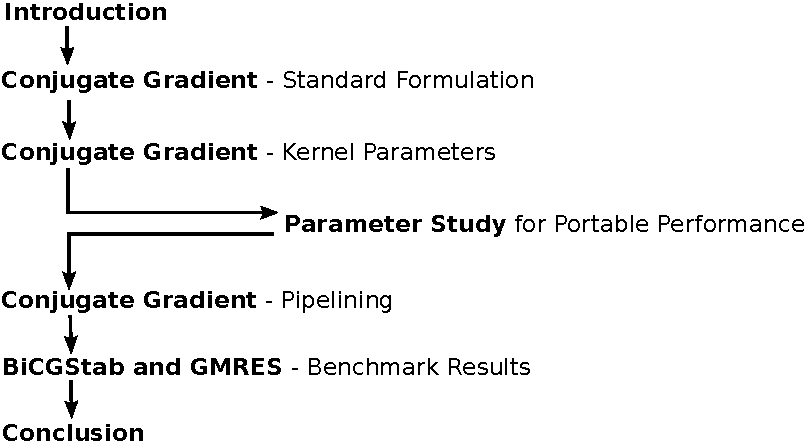
\includegraphics[width=0.9\textwidth]{figures/outline-crop}
 \end{center}
\end{frame}


\begin{frame}[fragile]{BiCGStab and GMRES}
 \begin{block}{BiCGStab}
 \begin{itemize}
  \item Similar to CG
  \item Two SpMV per iteration
  \item Pipelining: 4 kernel launches instead of 12
 \end{itemize}
 \end{block}   
 
 \begin{block}{GMRES}
 \begin{itemize}
  \item Store Krylov basis
  \item Orthonormalization in each step
  \item Pipelining: 3 kernel launches
 \end{itemize}
 \end{block}   

 \begin{block}{Benchmark Setup}
 \begin{itemize}
  \item Poisson equation in 2D
  \item GPUs from NVIDIA and AMD
 \end{itemize}
 \end{block}   

\end{frame}



\begin{frame}[fragile]{BiCGStab Benchmarks}
 \begin{block}{}
 \begin{center}
  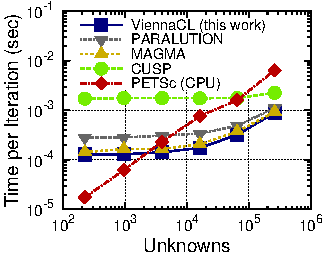
\includegraphics[width=0.7\textwidth]{figures/time-laplace2d-K20m-bicgstab}
 \end{center}
 \end{block}   
\end{frame}

\begin{frame}[fragile]{BiCGStab Benchmarks}
 \begin{block}{}
 \begin{center}
  \vspace*{-1cm}
  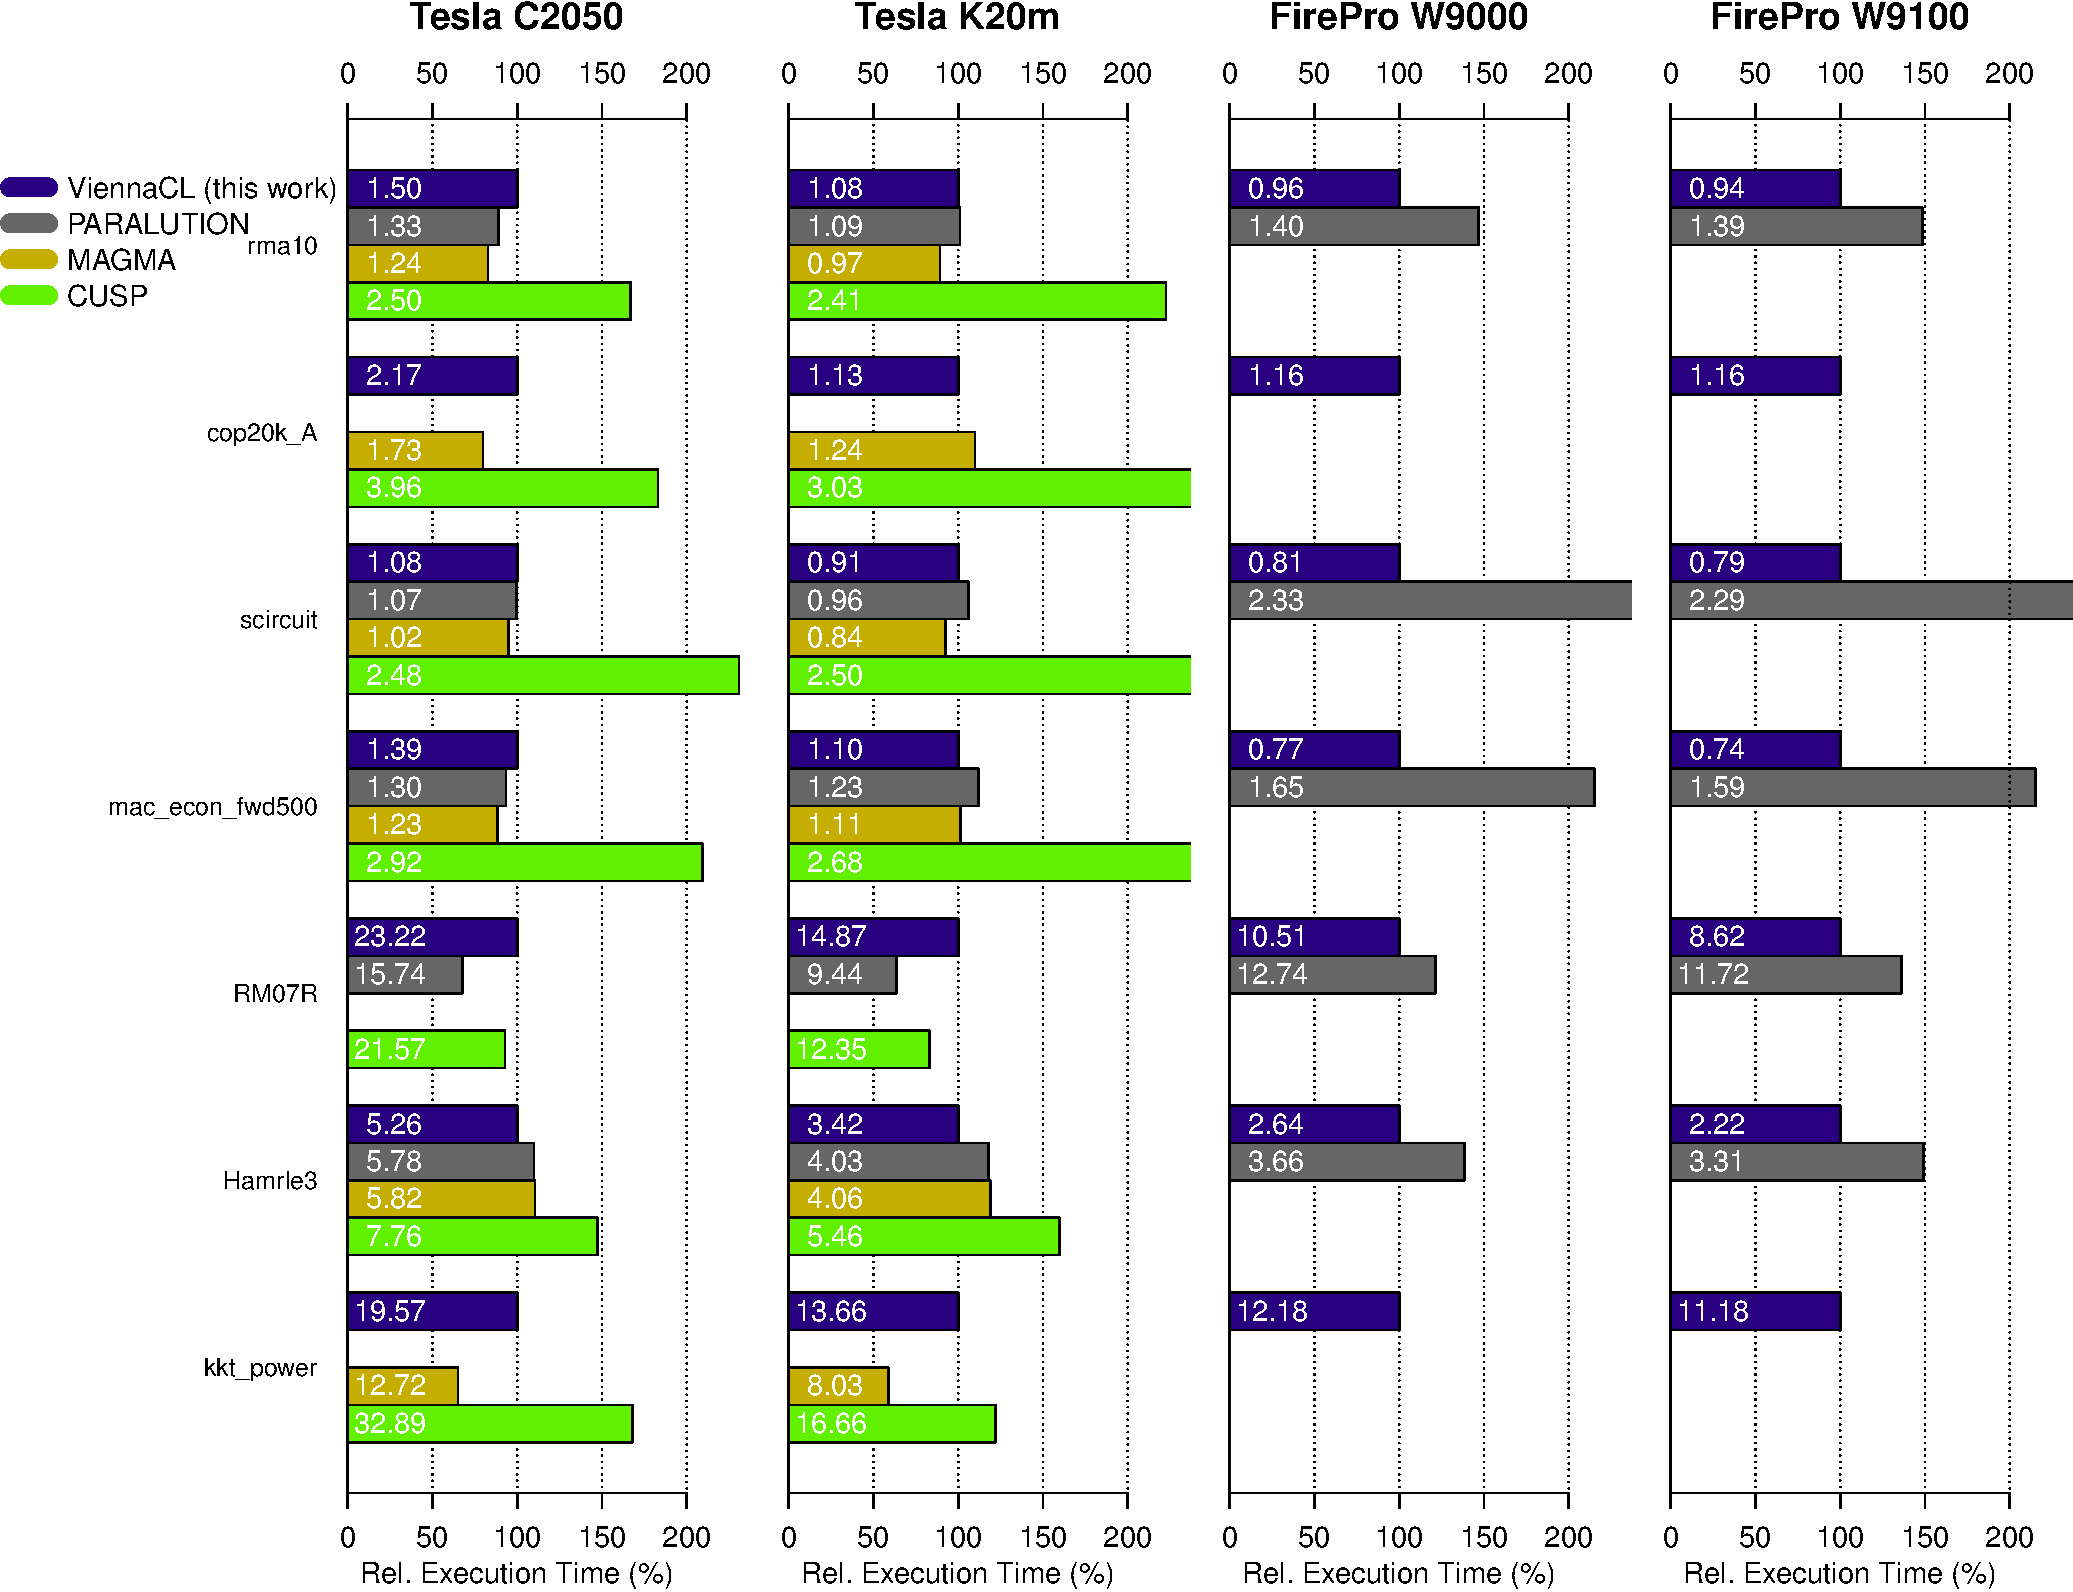
\includegraphics[width=0.9\textwidth]{figures/bicgstab}
 \end{center}
 \end{block}   
\end{frame}

\begin{frame}[fragile]{GMRES Benchmarks}
 \begin{block}{}
 \begin{center}
  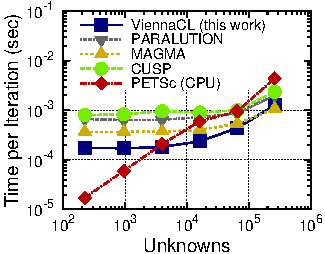
\includegraphics[width=0.7\textwidth]{figures/time-laplace2d-K20m-gmres}
 \end{center}
 \end{block}   
\end{frame}

\begin{frame}[fragile]{GMRES Benchmarks}
 \begin{block}{}
 \begin{center}
  \vspace*{-1cm}
  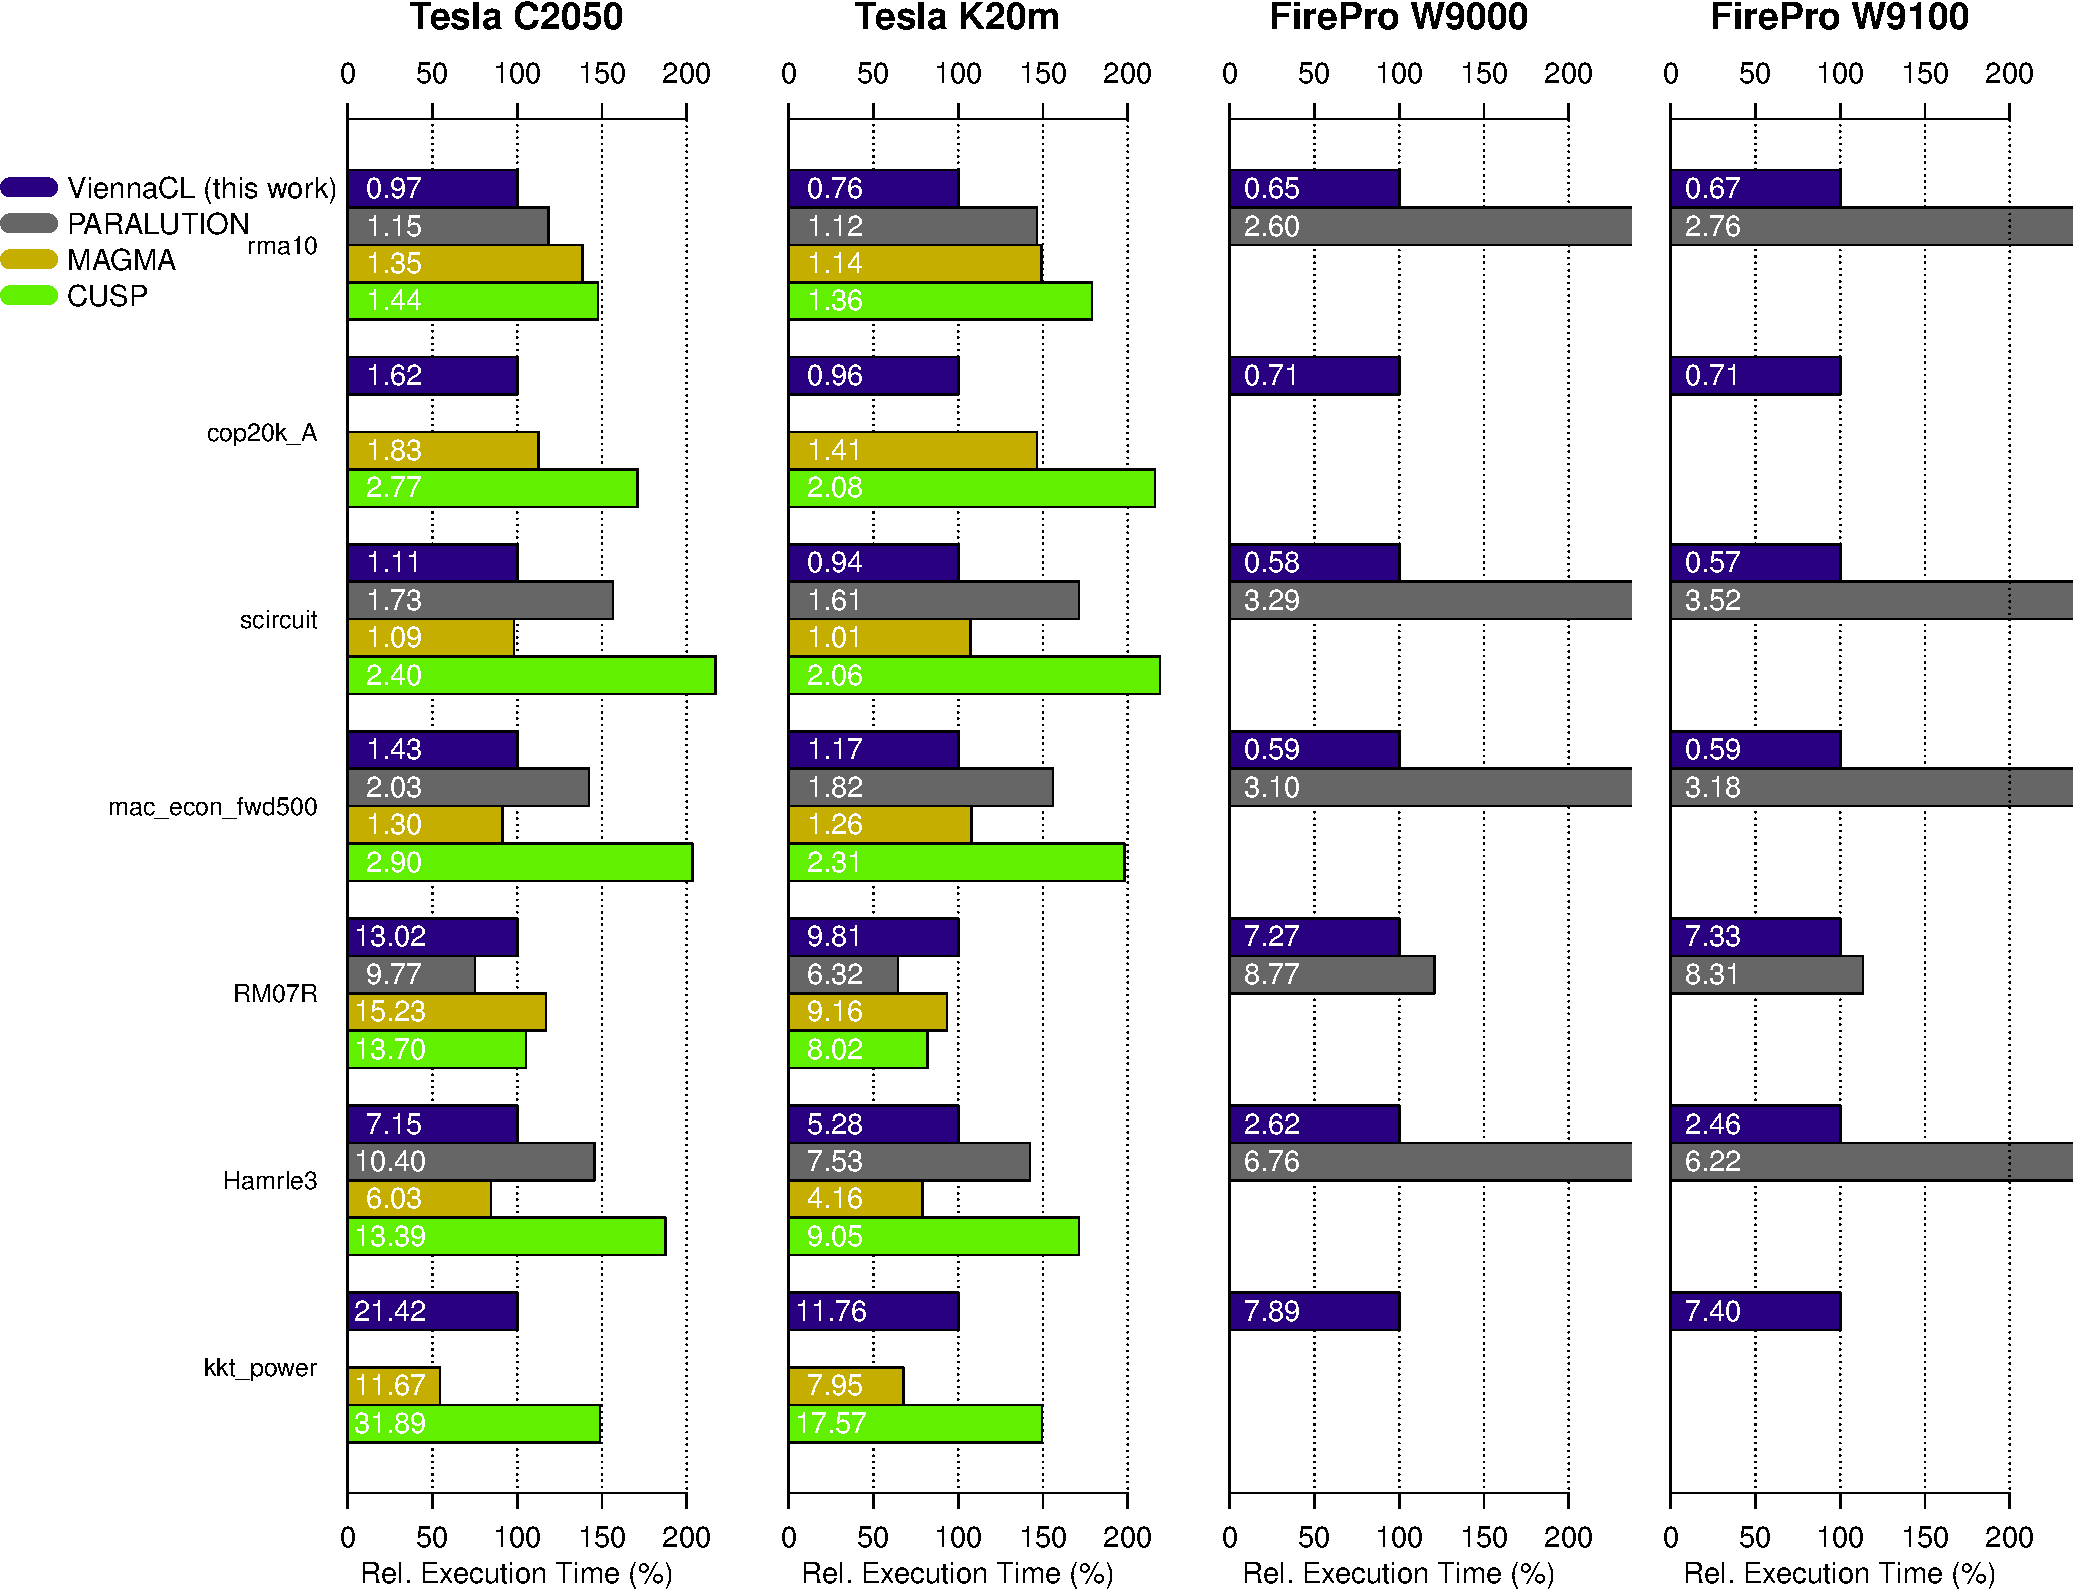
\includegraphics[width=0.9\textwidth]{figures/gmres}
 \end{center}
 \end{block}   
\end{frame}




%
% Community building
%

\begin{frame}{Outline}
 \begin{block}{ViennaCL Overview and Internals}\end{block}
 \begin{block}{Tuning Potpourri: Iterative Solvers}\end{block}
 \begin{block}{\textbf{Community Building}}\end{block}
 \begin{block}{Development Infrastructure}\end{block}
 \begin{block}{Miscellaneous}\end{block}
 \begin{block}{Summary}\end{block}
\end{frame}



\begin{frame}[fragile]{Community Building}

 \begin{block}{Recruiting Students}
  \begin{itemize}
   \item Projects for Bachelor's and Master's theses
   \item Summer internships (Google Summer of Code)
  \end{itemize}
 \end{block}

 \begin{block}{Working with Students}
  \begin{itemize}
   \item Benchmark for the project's documentation
   \item Add-on components rather than 'critical' features
   \item Continuous documentation
  \end{itemize}
 \end{block}

 
 \begin{block}{Project Organization}
  \begin{itemize}
   \item Version control!
   \item Modularize early
  \end{itemize}
 \end{block}
 

\end{frame}




\begin{frame}[fragile]{Community Building}

 \begin{block}{Public Communication}
  \begin{itemize}
   \item Private communication kills the community
   \item Mailing lists (e.g. sourceforge), IRC, ...
   \item Public developer meetings
  \end{itemize}
 \end{block}

 \begin{block}{Announce Releases}
  \begin{itemize}
   \item Social Media: Twitter, LinkedIn, Google+, ...
   \item Mailinglists: NA-Digest, etc.
   \item Provide a forum
   \item Changelog
   \item Information vs.~Annoyance
  \end{itemize}
 \end{block}

 
 \begin{block}{Other}
  \begin{itemize}
   \item Roadmap
   \item Provide repository write access early
   \item Be responsive (fast replies)
  \end{itemize}
 \end{block}
 

\end{frame}




%
% Development Infrastructure
%

\begin{frame}{Outline}
 \begin{block}{ViennaCL Overview and Internals}\end{block}
 \begin{block}{Tuning Potpourri: Iterative Solvers}\end{block}
 \begin{block}{Community Building}\end{block}
 \begin{block}{\textbf{Development Infrastructure}}\end{block}
 \begin{block}{Miscellaneous}\end{block}
 \begin{block}{Summary}\end{block}
\end{frame}




\begin{frame}[fragile]{Development Infrastructure}

 \begin{block}{Technical Must-Haves}
  \begin{itemize}
   \item Version control
   \item Build system (e.g. CMake)
   \item Nightly tests
   \item Compile cleanly at high warning levels
  \end{itemize}
 \end{block}

 \begin{block}{Recommended}
  \begin{itemize}
   \item Continuous integration
   \item Doxygen
   \item Coding style guide
  \end{itemize}
 \end{block}
 
 \begin{block}{Tools}
  \begin{itemize}
   \item Debugger
   \item Profiler
  \end{itemize}
 \end{block}
 
\end{frame}




%
% Miscellaneous
%

\begin{frame}{Outline}
 \begin{block}{ViennaCL Overview and Internals}\end{block}
 \begin{block}{Tuning Potpourri: Iterative Solvers}\end{block}
 \begin{block}{Community Building}\end{block}
 \begin{block}{Development Infrastructure}\end{block}
 \begin{block}{\textbf{Miscellaneous}}\end{block}
 \begin{block}{Summary}\end{block}
\end{frame}




\begin{frame}[fragile]{Expression Template Limitations}

 \begin{block}{Expression Templates are Not Enough}
  \begin{itemize}
   \item Consider
    \begin{lstlisting}
 u = x + y;
 v = x - y;
    \end{lstlisting}
   \item Suboptimal performance with almost any library
  \end{itemize}
 \end{block}
 
 \begin{center}
  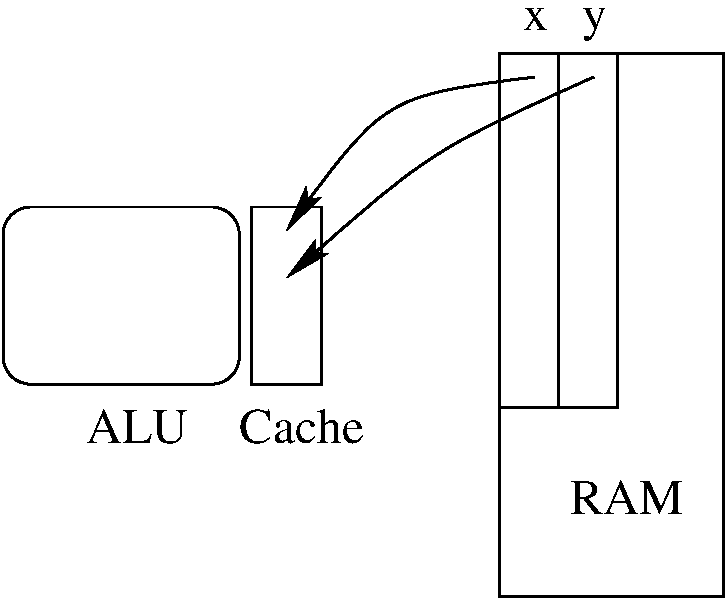
\includegraphics[width=0.4\textwidth]{kernel-fusion-1.pdf}
 \end{center}


\end{frame}



\begin{frame}[fragile]{Expression Template Limitations}

 \begin{block}{Expression Templates are Not Enough}
  \begin{itemize}
   \item Consider
    \begin{lstlisting}
 u = x + y;
 v = x - y;
    \end{lstlisting}
   \item Suboptimal performance with almost any library
  \end{itemize}
 \end{block}
 
 \begin{center}
  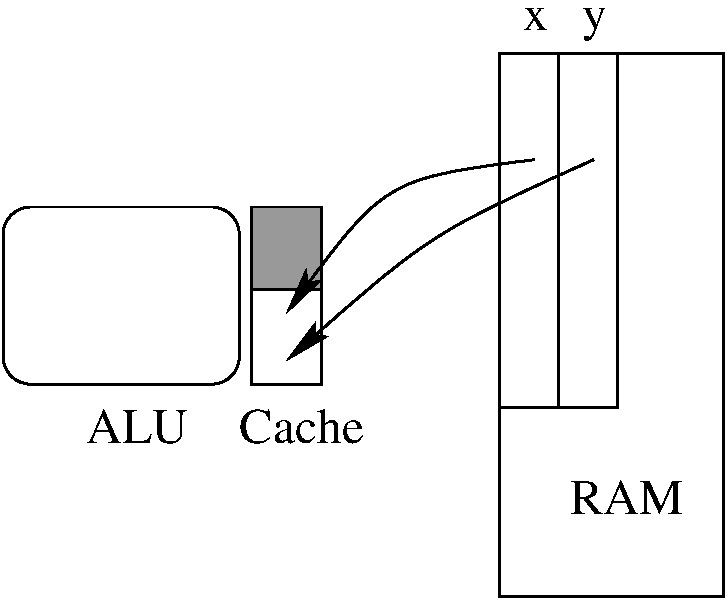
\includegraphics[width=0.4\textwidth]{kernel-fusion-2.pdf}
 \end{center}


\end{frame}


\begin{frame}[fragile]{Expression Template Limitations}

 \begin{block}{Expression Templates are Not Enough}
  \begin{itemize}
   \item Consider
    \begin{lstlisting}
 u = x + y;
 v = x - y;
    \end{lstlisting}
   \item Suboptimal performance with almost any library
  \end{itemize}
 \end{block}

 \begin{block}{OpenCL Kernel Generation}
   \begin{itemize}
    \item Separate temporary avoidance from operation execution
    \begin{lstlisting}
 viennacl::kernel_fusion(true); //API not final!
 u = x + y;
 v = x - y;
 ...
 viennacl::kernel_fusion(false);
    \end{lstlisting}
    \item Semi-transparent kernel fusion in preparation (scheduler)
   \end{itemize}
 \end{block}
\end{frame}


\begin{frame}{Expression Template Limitations}

 \begin{block}{Benchmark Results}
  \begin{center}
   $\beta \leftarrow x^T \cdot (2x + y)$ \\
   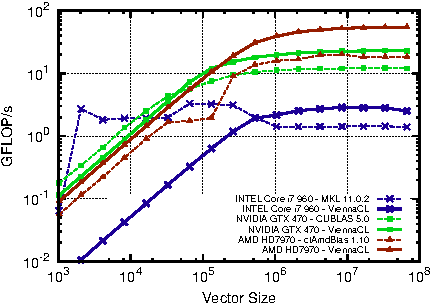
\includegraphics[width=0.75\textwidth]{figures/daxpy_ddot.pdf} \\
  \end{center}
   \scriptsize Tillet \textit{et al.}, HotPar '13

 \end{block}

\end{frame}




\begin{frame}[fragile]{OpenCL on the CPU}

 \begin{block}{Cost of a Function Call}
  \begin{itemize}
   \item Plain C: Tens of nanoseconds
   \item OpenCL: Several microseconds
  \begin{lstlisting}
     std::vector<double>      std_x(100);
viennacl::vector<double>      vcl_x(100);

for (size_t i=0; i<100; ++i){
    std_x[i] = rand();
    vcl_x[i] = rand();  //possible, inefficient
}
\end{lstlisting}
  \end{itemize}
 \end{block}

 \begin{block}{Host-based Execution}
  \begin{itemize}
   \item Required for serial code
   \item Rich library set
  \end{itemize}
 \end{block}

 \begin{block}{Recommendation}
  \begin{itemize}
   \item Don't use OpenCL for CPUs
  \end{itemize}
 \end{block}
 
\end{frame}





\begin{frame}[fragile]{Iterators}

 \begin{block}{C++ Loves Iterators}
  \begin{itemize}
   \item Fundamental for STL
   \item Forward Iterator vs. Random Access Iterator
    \begin{lstlisting}
 std::copy(x.begin(), x.begin() + 5, y.begin() + 4);
    \end{lstlisting}
  \end{itemize}
 \end{block}

 \pause
 \begin{block}{Massive Parallelism}
  \begin{itemize}
   \item Forward Iterator is sequential by nature
   \item Only Random Access Iterator suitable for parallelism
   \item Simpler APIs:
    \begin{lstlisting}
 x[range(0, 5)] = y[range(4, 9)];
    \end{lstlisting}
  \end{itemize}
 \end{block}
 
\end{frame}





%
% Conclusion:
%
\begin{frame}{Summary and Conclusion}

  \begin{block}{ViennaCL}
   \begin{itemize}
    \item Convenient high-level linear algebra library
    \item CUDA-, OpenCL-, and OpenMP-backends
    \item 
     \begin{center}
      \Large http://viennacl.sourceforge.net/
     \end{center}
   \end{itemize}
  \end{block}

  %\pause
  \begin{block}{Using Heterogeneous Systems}
   \begin{itemize}
    \item Reuse software libraries
    \item 'Time to science' most important
   \end{itemize}
  \end{block}
  
  %\pause
  \begin{block}{Slides}
    \begin{itemize}
     \item Available in folder PHSP2014 at
     \begin{center}
      \Large http://github.com/karlrupp/slides
     \end{center}
    \end{itemize}
  \end{block}

\end{frame}

